\documentclass[10pt]{article}
\usepackage{titling}
\usepackage{lipsum}
\usepackage{amsmath}
\usepackage{listings}
\usepackage{graphicx}
\usepackage{subcaption}
\usepackage{multicol}
\usepackage{pgfplots}
\usepackage[margin=0.5in]{geometry}

\pagestyle{empty}
% Final Exam

% Wednesday, June 7 at 1 - 3 pm
% comprehensive - covers all the materials we discussed in class
% closed book and notes
% you may bring three formula sheets - two 8.5x11' pieces of paper with notes on both sides allowed
% statistical tables will be provided
% practice problem set to be posted by Friday, June 2
% office hour on Tuesday at 1 - 3 pm
\begin{document}
\subsection*{Blocking in $2^k$ Design}
\hrule width \textwidth
\vspace{6pt}
Assume: 1 observation per cell. no interaction between blocks and treatments. \\
Model: \\
$y_{ijklm} = \tau_i + \beta_j + \gamma_k 
           + (\tau \beta)_{ij} + (\tau \gamma)_{ik} + (\beta \gamma)_{jk}
           + (\tau \beta \gamma)_{ijk} + \mathcal{B}_l + \epsilon_{ijklm}$ \\

\begin{multicols}{2}
  \begin{flushleft}
    \textbf{$2^3$ With Blocking - ANOVA}
    \begin{equation*}
      \begin{array}{c|c}
        \text{Source} & \text{df}\\
          \hline
          \text{Model} & 8 \\
          \text{A} & 1 \\
          \text{A} & 1 \\
          \text{AB} & 1\\
          \vdots & \vdots \\
          \text{ABC} & 1\\
          \text{Blocks} & b - 1 \\
          \text{Error} & df_{total} - (df_{model} + df_{blocks})  \\
          \hline
          \text{Total} & 8b - 1 \\
      \end{array}
    \end{equation*}
  \end{flushleft}
\end{multicols}

\textbf{Contrast Constants}
\begin{figure}[h] % IMAGE FIGURE
  \centering
  \includegraphics[width=0.8\textwidth, height=.25\textheight]{./images/table.png}
  \label{fig:interaction}
\end{figure}

\textbf{Interaction Plot}
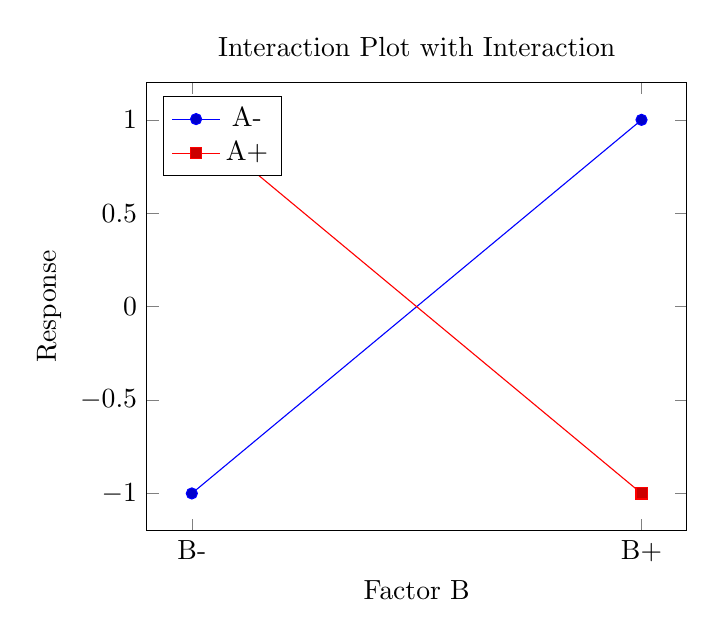
\begin{tikzpicture}
  \begin{axis}[
      title={Interaction Plot with Interaction},
      xlabel={Factor B},
      ylabel={Response},
      symbolic x coords={B-, B+},
      xtick=data,
      legend pos=north west
  ]
  \addplot coordinates {(B-, -1) (B+, 1)};
  \addplot coordinates {(B-, 1) (B+, -1)};
  \legend{A-,A+}
  \end{axis}
  \end{tikzpicture}

Main effect of $A = \frac{\bar{y}_{ab} + \bar{y}_a}{2} - \frac{\bar{y}_{b} + \bar{y}_{(1)}}{2}$. Main effect of $B = \frac{\bar{y}_{ab} + \bar{y}_b}{2} - \frac{\bar{y}_{a} + \bar{y}_{(1)}}{2}$. Interaction effect $AB = \frac{(\bar{y}_{ab} - \bar{y}_b) - (\bar{y}_a - \bar(y_{(1)}))}{2}$ \\

Effect of $B$ at $A^{+} = \mu_{ab} - \mu_{a}$.


\end{document}
